\documentclass[10pt,conference,compsocconf]{IEEEtran}

\usepackage[utf8]{inputenc}
\usepackage{amsmath,amssymb,amsthm}
\usepackage{graphicx}
\usepackage{booktabs}
\usepackage{tabularx}
\usepackage[table]{xcolor}
\usepackage{colortbl}
\usepackage{contour}
\contourlength{0.8pt} % thickness of the halo
\usepackage{url}
\ifCLASSOPTIONcompsoc
  \usepackage[nocompress]{cite}
\else
  \usepackage{cite}
\fi
\usepackage{enumitem}
\usepackage{algorithm}
\usepackage{algpseudocode}
\usepackage{pgf-pie}
\usepackage{pgfplots}
\usepgfplotslibrary{dateplot}
\usepgfplotslibrary{units}
\pgfplotsset{compat=1.18}
\usepackage{comment}
\usepackage{capt-of}
\usepackage[obeyclassoptions,mode=buildnew]{standalone}

\usetikzlibrary{arrows.meta, positioning, calc}

% darken the colors a little bit
\definecolor{red}  {rgb}{0.9,0.0,0.0}
\definecolor{green}{rgb}{0.0,0.7,0.0}
\definecolor{blue} {rgb}{0.0,0.0,0.9}

\definecolor{OkabeBlue}{RGB}{0,114,178}
\definecolor{OkabeOrange}{RGB}{213,94,0}
\definecolor{OkabeGreen}{RGB}{0,158,115}
\definecolor{OkabeSky}{RGB}{86,180,233}
\definecolor{OkabeVermilion}{RGB}{230,159,0}

\definecolor{OIblue}{HTML}{0072B2}
\definecolor{OIorange}{HTML}{E69F00}
\definecolor{OIgrey}{HTML}{999999}

\newcommand{\discuss}[1]{\textcolor{blue}{#1}}
\newcommand{\red}[1]{\textcolor{red}{#1}}
\newcommand{\blue}[1]{\textcolor{green}{#1}}
\newcommand{\edited}[1]{\textcolor{blue}{#1}}
\newcommand{\ori}[1]{\textcolor{blue}{Ori: #1}}

\newif\ifshowaradnotes
\showaradnotesfalse
\newcommand{\arad}[1]{%
  \ifshowaradnotes\par\noindent\textcolor{orange}{\textbf{ARAD NOTE:} #1}\par\fi}

% Numbers quoted in the text, generated from the experiment results by make_paper_assets.py
% Generated by make_paper_assets.py from the experiment results; do not edit by hand.
\newcommand{\NPools}{27}
\newcommand{\NFamilies}{21}
\newcommand{\SensitivityK}{3}
\newcommand{\DataEnd}{October~27,~2026}
\newcommand{\NHours}{1{,}028{,}290}
\newcommand{\NDecisions}{52}
\newcommand{\EligibleMin}{17}
\newcommand{\EligibleMax}{27}
\newcommand{\FeePositions}{4{,}104}
\newcommand{\FeeIntervals}{5{,}817}
\newcommand{\FeeMedianErr}{0.035\%}
\newcommand{\FeeWithinFive}{99.1\%}
\newcommand{\SwapErrFull}{0.7\%}
\newcommand{\SwapErrFive}{1.1\%}
\newcommand{\SwapErrOne}{6.4\%}
\newcommand{\MeanIL}{-0.38\%}
\newcommand{\MeanPredIL}{-0.37\%}
\newcommand{\LvrSlope}{1.11}
\newcommand{\LvrRsq}{0.42}
\newcommand{\CorrOffset}{91\%}
\newcommand{\CorrRho}{0.93}
\newcommand{\ModelTailRate}{10.6\%}
\newcommand{\ModelTailKupiec}{0.46}
\newcommand{\EmpTailRate}{15.9\%}
\newcommand{\NetTailRate}{20.2\%}
\newcommand{\IcLvr}{0.27}
\newcommand{\IcLvrT}{13.3}
\newcommand{\IcNetTail}{-0.09}
\newcommand{\IcNetTailT}{-2.1}
\newcommand{\IcLowVar}{-0.27}
\newcommand{\NLvrTestsSig}{3}
\newcommand{\NLvrTests}{9}
\newcommand{\NSensCells}{81}
\newcommand{\NSensNetTailBehind}{76}
\newcommand{\MainK}{3}
\newcommand{\AbsLvrMean}{0.70\%}
\newcommand{\AbsNetTailMean}{0.44\%}
\newcommand{\AbsGainVsNetTail}{58\%}
\newcommand{\AbsCvarCut}{38\%}
\newcommand{\AbsReturnKept}{88\%}
\newcommand{\IcRangeOne}{0.06}
\newcommand{\IcRangeFive}{0.11}
\newcommand{\IcRangeTwenty}{0.22}
\newcommand{\IcRangeSigmaMin}{0.21}
\newcommand{\IcRangeSigmaMax}{0.26}
\newcommand{\IcRangeOneTail}{0.13}
\newcommand{\LamMax}{5}
\newcommand{\IcRangeNetTailMax}{0.07}
\newcommand{\NetRangeOne}{-1.09\%}
\newcommand{\NetRangeTwenty}{-0.22\%}
\newcommand{\NetRangeSigma}{0.31\%}
\newcommand{\SigmaRangeMax}{3}
\newcommand{\HalfLifeMin}{5}
\newcommand{\HalfLifeMax}{223}


\usepackage[most]{tcolorbox}
\pagestyle{plain}
\title{Mitigating DeFi Impermanent Loss through Risk-Aware Pool Screening}
\thispagestyle{empty}
%\author{\IEEEauthorblockN{Anonymous Authors}}

\author{
\IEEEauthorblockN{Arad Kotzer and Ori Rottenstreich}
\IEEEauthorblockA{
Technion %- Israel Institute of Technology
}
}

\begin{document}

\maketitle

\begin{abstract}
Liquidity provision in automated market makers is widely pursued as a passive income strategy. However, impermanent loss (IL) frequently causes it to underperform simple buy-and-hold portfolios. Whether a pool is worth supplying depends jointly on the fees it pays and on how far the prices of its two tokens are likely to drift apart. In this paper, we propose a risk-aware pool-screening framework that weighs fee income against an explicit model of this divergence risk. The model captures both the expected loss, which grows with the volatility of the pair's relative price, and the risk of rare large losses, while a single risk-aversion parameter sets the balance between return and downside protection. We evaluate the framework out of sample on 27 Uniswap v3 pools over more than five years, including transaction costs. Correlated token pairs do suffer less IL, as theory predicts, but liquidity providers crowd into these low-risk pools until their fees shrink by a similar margin. Ranking pools by divergence risk alone therefore favors pools that earn almost nothing, whereas weighing fees against the expected loss consistently identifies the more profitable pools. Holding the three pools with the best balance of fees and expected loss earns 0.70\% per month over buy-and-hold after costs, 58\% more than a purely empirical tail-adjusted score. Our tail-risk forecast is well calibrated. A moderate penalty on it cuts the average loss in the worst months by 38\% while keeping 88\% of the return.
\end{abstract}


\begin{IEEEkeywords}
Blockchain, DeFi, Impermanent Loss
\end{IEEEkeywords}

\section{Introduction}

The Decentralized Finance (DeFi) ecosystem comprises various financial services that run as blockchain applications~\cite{schar2021decentralized, zetzsche2020decentralized, jensen2021introduction, Bitcoin, wood2014ethereum}. DeFi enables participants to earn yield by providing services. The core strategies revolve around lending money for interest and providing liquidity to token exchanges for transaction fees. They also include generating actions on DeFi platforms to earn engagement rewards. Recent estimates of the DeFi token market cap range from approximately 90 billion USD~\cite{forbes2025defi} to 103 billion~\cite{coingecko2025defi}, as of December 2025.

However, the prevailing narrative that liquidity provision is a passive yield farming strategy is increasingly challenged by the reality of \textit{Impermanent Loss} (IL). IL represents the shortfall between the value of the pool position of a Liquidity Provider (LP) and the value of simply holding the same tokens (HODL). When the relative price of the two assets moves away from its initial level, the Automated Market Maker (AMM) automatically adjusts the pool’s reserve composition to satisfy its pricing rule.
By doing so, it sells the outperforming asset and buys the underperforming one.
As a result, the LP's total position value can end up below what they would have obtained by simply holding the assets outside the pool.

Empirical evidence suggests that for many LPs, the fee income generated is insufficient to compensate for this structural drag.
Loesch et al.~\cite{loesch2021impermanent} study 17 popular Uniswap v2 pools and show that total fees earned (199M USD) failed to offset IL, resulting in an aggregate underperformance of 61M USD compared to the potential revenue of the HODL strategy (261M USD).
These results imply a yield trap, as headline APYs look attractive, though after subtracting IL, fees often don’t cover the loss.

In this paper, \textit{we present a risk-aware LP pool-screening framework that weighs fee compensation against an explicit model of divergence risk}.
An LP's holding in a pool is called a \emph{position}. It consists of the deposited tokens, which the AMM rebalances as prices move, and the fees earned on them. In Uniswap v2, every position supplies liquidity at all prices, whereas Uniswap v3 lets the LP choose the price range in which its liquidity is active. We base our model on a \emph{full-range} position, which is active at all prices and therefore always earns fees. For such a position, both sides of the tradeoff can be measured consistently. Fees follow exactly from the pool's on-chain fee counters, and the expected divergence loss equals the loss-versus-rebalancing (LVR) rate $\sigma^2_{\text{pair}}/8$~\cite{milionis2022automated}, where $\sigma^2_{\text{pair}}$ is the variance of the pair's log price. Correlation between the two tokens enters through $\sigma^2_{\text{pair}}=\sigma_A^2+\sigma_B^2-2\rho\cdot\sigma_A\cdot\sigma_B$, where $\sigma_A$ and $\sigma_B$ are the volatilities of the two tokens and $\rho$ is their correlation. We complement the expected loss with a tail forecast derived from hourly realized volatility, and combine both into a single score with a risk-aversion parameter $\lambda$.

We focus empirically on Uniswap v3 as it is widely used and because concentrated liquidity provides a demanding setting in which to test when full-range metrics remain informative. The model itself is not specific to Uniswap v3. A full-range v3 position follows the same constant-product rule as a Uniswap v2 position, so the score applies to v2 pools directly, with fees measured from the growth of the pool reserves instead of fee counters. Uniswap v4 keeps the concentrated-liquidity mechanics and fee counters of v3, so the same measurement applies there as well. Because fees are measured from what the pool actually paid rather than from its fee tier, this also covers v4 pools whose hooks set dynamic fees, as long as the hook does not change the pricing rule itself.

We apply the framework to 27 Uniswap v3 pools over more than five years. Correlated pairs indeed suffer far less IL than stable--volatile pairs, with a mean monthly loss of 0.07\% compared with 0.45\%. However, their fees are lower by a similar factor, 0.09\% compared with 0.45\% per month. This is consistent with competition among LPs, who crowd into low-risk pools until the fees no longer exceed the risk. As a result, ranking pools by divergence risk alone selects pools that earn almost nothing, and a useful score must weigh both sides of the tradeoff. Building on these observations, the main contributions of this paper are as follows.
\begin{itemize}[leftmargin=*,itemsep=1pt,topsep=2pt]
    \item We present a consistent fee and divergence model for full-range positions and validate it against \FeePositions{} real on-chain positions (median fee error \FeeMedianErr{}) and swap-level replays.
    \item We propose a mean--tail screening score $S_\lambda$ whose tail term is a model-based IL quantile. Unlike the empirical quantile, it passes standard coverage tests.
    \item We evaluate the score out of sample over \NPools{} pools with eligibility filters and costs, and show that the LVR-based score ranks pools well and that a small $\lambda$ reduces downside risk while retaining most of the return.
\end{itemize}
Table~\ref{tab:notation} summarizes the main notation used throughout the paper.


\begin{table}[t]
\centering
\caption{Summary of notation.}
\label{tab:notation}
\scriptsize
\begingroup
\setlength{\tabcolsep}{3pt}
\renewcommand{\arraystretch}{0.92}
\begin{tabular}{@{}p{0.35\columnwidth}p{0.59\columnwidth}@{}}
\toprule
Notation & Description \\
\midrule
$p_t$, $R=p_{t_1}/p_{t_0}$, $x=\ln R$
& Pool price, price ratio, and log price change. \\

$\mathrm{IL}(R)$
& Full-range CPMM IL. \\

$G^{0}_t$, $G^{1}_t$, $L$
& Fee-growth accumulators and position liquidity. \\

$y^{\mathrm{fee}}$, $\sigma^2$
& Fee yield and realized variance of the log price over a period. \\

$\sigma^2_{\text{pair}}$, $\rho$
& Pair variance and correlation of the two tokens. \\

$q$, $\mathrm{IL}_q$
& Tail level and model-based $q$-quantile of IL. \\

$S_\lambda$, $\lambda$
& Mean--tail screening score and risk aversion. \\

$\mathrm{Net90}$
& Empirical tail-adjusted score. \\

\bottomrule
\end{tabular}
\endgroup
\end{table}

\section{Background and Related Work}
\label{sec:background}

\subsection{AMM (Automated Market Maker)}
Automated market makers (AMMs)~\cite{hertzog2017bancor} are decentralized exchange protocols that execute token swaps against liquidity pools according to predefined pricing rules. This paper focuses on the constant-product market maker (CPMM), whose reserves satisfy $x_0\cdot x_1=K$, as implemented by Uniswap v2. Uniswap v3 retains the constant-product structure but allows liquidity providers to concentrate liquidity within selected price ranges. Within an active range, a position behaves like a CPMM with virtual reserves, while outside the range it becomes inactive and holds only one of the two tokens. Other invariant-based AMM designs include Balancer's weighted geometric-mean model and Curve's stableswap model~\cite{bartoletti2022theory}.

AMMs operate as continuous, on-chain price discovery mechanisms driven by arbitrage flow. Whenever the pool price deviates from external markets, arbitrage restores alignment~\cite{angeris2020improved}.
Hence, arbitrage creates a stabilizing mechanism and a source of value extraction~\cite{pusceddu2024lean}.
This arbitrage-based alignment sustains on-chain liquidity and also determines value transfers.

\subsection{Liquidity Provision}
\label{sec:liquidity-provision}

Liquidity provision refers to users depositing tokens into an AMM pool, enabling traders to swap assets directly against pooled reserves. In return, \textit{liquidity providers} (LPs) receive a proportional share of the pool’s swap fees~\cite{gogol2024sok, chiu2023fragility, saengchote2023decentralized}.
For example, in a pool of Uniswap v2 ETH / USDC, LPs deposit equal values of ETH and USDC. Traders then exchange one asset for the other via the constant product invariant of the pool. This mechanism underpins decentralized exchanges by providing continuous on-chain liquidity without order books.

\subsubsection{Fee microstructure and concentrated liquidity}
AMM protocols differ in how fees interact with liquidity.
In Uniswap v2, swap fees are \emph{reinvested into the pool reserves} on each trade, so the product $x_0 \cdot x_1{=}K$ grows.
In Uniswap v3, fees are added to the \emph{separate fee counters} of each position and do not change the active liquidity or the reserves until the LP explicitly claims or reinvests them.
Moreover, v3 allows LPs to choose a price band $[p_{-},p_{+}]$ and provide liquidity only inside it.
Let $p_{\text{pool}}$ denote the instantaneous pool price implied by reserves, defined as
$p_{\text{pool}} = x_1/x_0$.
When $p_{\text{pool}}\in[p_{-},p_{+}]$, the position behaves locally like a CPMM with ``virtual'' reserves determined by $[p_{-},p_{+}]$ and its liquidity $L$, and it earns fees.
If price exits this band, the position becomes out of range and is held entirely in a single asset, $c_0$ when $p_{\text{pool}}<p_{-}$ and $c_1$ when $p_{\text{pool}}>p_{+}$.
In this out-of-range state, the position provides no active liquidity and therefore accrues no fees until the price re-enters the range or the LP rebalances.
The pool tracks the fees earned per unit of in-range liquidity in two cumulative accumulators, $\texttt{feeGrowthGlobal0X128}$ and $\texttt{feeGrowthGlobal1X128}$ (one per token), from which each position's fees are settled.


\subsection{Impermanent Loss}
\label{sec:background_il}

\emph{Impermanent Loss} (IL) is the fundamental risk for liquidity providers in AMMs. It is the relative underperformance of an LP's pool position versus a passive buy-and-hold (\emph{HODL}) strategy with the same initial assets~\cite{evans2021liquidity, aoyagi2020liquidity}.


\subsubsection{Mechanism and Formalization}
IL arises from the convex payout structure of the AMM invariant. When the relative market price of the pooled tokens changes, arbitrageurs trade against the pool to realign its internal price with external markets. This process forces the AMM to sell the appreciating asset and buy the depreciating asset, systematically reducing the total value of the pool relative to the HODL benchmark.
For a standard CPMM like Uniswap v2, where reserves $x_0, x_1$ satisfy $x_0 \cdot x_1 = K$, Tiruviluamala et al.~\cite{tiruviluamala2022general} derived the canonical closed-form expression for IL as a function of the price ratio change $R = p'/p$:
\begin{equation}
    \mathrm{IL}(R) = \frac{2\sqrt{R}}{1+R} - 1.
    \label{eq:il_canonical}
\end{equation}
This function is always non-positive ($\mathrm{IL} \le 0$) and symmetric with respect to log-returns, implying that LPs incur losses regardless of the direction of price divergence. While the loss is referred to as impermanent because it theoretically vanishes if prices return to their initial ratio (namely, $IL(R)=0$ for $R=1$), the path-dependent nature of volatility often crystallizes these losses upon withdrawal.

\subsubsection{Empirical Severity}
Empirical studies confirm that $IL \le 0$ is a pervasive feature of AMM liquidity provision, while the ability of fees to offset it depends on pool type and market conditions.
For Uniswap v2, stablecoin pairs tend to exhibit mild IL, whereas volatile or exotic pairs often experience IL that exceeds fee income~\cite{heimbach2021behavior, boueri2021g3m}.
In Uniswap v3, concentrated liquidity can amplify divergence exposure, and passive narrow-range positions in volatile pools frequently realize net losses~\cite{heimbach2022risks}.
Fee-aware analyses report that small price fluctuations can yield impermanent gain when fee flow is sufficiently strong, but this cushioning is limited under large divergence moves~\cite{roman2025impact}.


\subsection{Related Work}
Prior work studies LP risk in AMMs through IL theory and empirical evaluations across protocols.
Canonical results derive closed-form IL for constant-product pools and extend it to broader invariant-based and multi-asset AMM designs~\cite{tiruviluamala2022general}.
Measured underperformance depends on the chosen benchmark and, in Uniswap v3, on concentrated-liquidity mechanics, which make outcomes range-dependent and may leave positions out of range~\cite{aigner2021uniswap,loesch2021impermanent,heimbach2022risks}.
Related perspectives replace HODL with rebalancing-based benchmarks, such as loss-versus-rebalancing (LVR), and derive the fee levels required to compensate LPs fairly~\cite{milionis2022quantifying,milionis2022automated,cohen2023inefficiency}.
Recent work further shows that accounting for fees can materially change conclusions about LP profitability~\cite{roman2025impact} and introduces relative value and fee-adjusted relative value measures for comparing outcomes across AMM designs~\cite{tangri2023generalizing}.
Our work builds on the LVR rate as the expected divergence cost, and turns it into an ex-ante pool-selection rule with a calibrated tail term, evaluated out of sample.


\section{Fee and Divergence-Risk Model}
\label{sec:metrics}

Recall from Section~\ref{sec:background_il} that IL depends on the change of the relative price over the holding period. This change is unknown when the LP supplies liquidity. Hence, an LP choosing a pool has to forecast both the fees and the divergence loss over the holding horizon. We model both for a \emph{full-range} position, which is always in range and for which the CPMM formula~\eqref{eq:il_canonical} is exact in Uniswap v3. We use the resulting quantities as ex-ante screening scores, and Section~\ref{subsec:robustness} tests them for concentrated ranges.

\subsection{Fee Accounting}
\label{subsec:fee_accounting}
Uniswap v3 tracks fees per unit of liquidity rather than per position~\cite{uniswapv3}. For each token $i\in\{0,1\}$, the pool keeps a fee-growth accumulator $G^{i}_t$, which sums the fees paid in token~$i$ per unit of in-range liquidity since the pool was created.\footnote{The contract stores $G^{i}_t$ as an integer equal to its value multiplied by $2^{128}$, as the EVM has no fractional numbers. We divide it by $2^{128}$ before use.} Since a full-range position is always in range, a position with liquidity $L$ held from $t_0$ to $t_1$ earns exactly
\begin{equation}
\label{eq:fee_growth}
F^{i}_{t_0:t_1} = L\cdot\bigl(G^{i}_{t_1}-G^{i}_{t_0}\bigr), \qquad i\in\{0,1\}.
\end{equation}
We value both fee amounts at the closing price and divide them by the HODL value, which gives the fee yield $y^{\mathrm{fee}}$. A common shortcut estimates this yield as $\mathrm{FeeTier}\cdot\mathrm{Volume}/\mathrm{TVL}$. However, TVL also counts liquidity that is out of range and earns nothing. Eq.~\eqref{eq:fee_growth} counts only the liquidity that was in range at each swap, so fees and IL refer to the same position. For a concentrated range, we credit the accumulator only in hours in which the price lies inside the range.

Eq.~\eqref{eq:fee_growth} assumes that the position is small relative to the pool, so adding it does not change the fees that traders pay. This assumption fails when little liquidity is in range. For instance, a swap that pushes the price through nearly empty ticks makes $G^{i}$ jump. A large hypothetical position would then be credited more fees than all traders actually paid. To prevent this, we cap the fees of the position in each UTC day at the total fees that the pool collected on that day.

\subsection{Expected Divergence Loss}
\label{subsec:lvr}
Let $x=\ln R$ be the log price change over the horizon and $\sigma^2$ its variance. For small moves, a second-order expansion of Eq.~\eqref{eq:il_canonical} gives $\mathrm{IL}(e^{x}) = \operatorname{sech}(x/2)-1 \approx -x^2/8$. Intuitively, IL grows with the square of the price move. For instance, a 10\% rise in the relative price costs the LP 0.11\%, while a 50\% rise costs 2.0\%. Taking the expectation gives
\begin{equation}
\label{eq:lvr}
\mathbb{E}[\mathrm{IL}] \approx -\frac{\sigma^2}{8},
\end{equation}
which coincides with the LVR rate of a constant-product pool~\cite{milionis2022automated}. Hence, the expected loss is one eighth of the variance of the relative price. For instance, a monthly volatility of 10\% ($\sigma^2=0.01$) implies an expected loss of 0.125\% per month.

We estimate $\sigma^2$ as the realized variance of the hourly log pool price, namely the sum of the squared hourly log returns over the period. We use hourly rather than minute prices for two reasons. First, the subgraph aggregates pool data per hour. Additionally, at finer frequencies the measured variance is dominated by market microstructure noise~\cite{ait2005often}. Swaps move the pool price away from external markets and arbitrageurs move it back, and this back-and-forth inflates the variance of minute returns. A month still contains about 720 hourly returns, which is enough for a precise estimate.

The pair variance decomposes as
\begin{equation}
\label{eq:pair_variance}
\sigma^2_{\text{pair}} = \sigma_A^2 + \sigma_B^2 - 2\rho\cdot\sigma_A\cdot\sigma_B,
\end{equation}
where $\sigma_A^2$ and $\sigma_B^2$ are the USD variances of the two tokens and $\rho$ is their correlation. Eq.~\eqref{eq:pair_variance} explains why correlated pairs suffer less IL, as the covariance term offsets most of the individual variances. For instance, two tokens with a monthly volatility of 20\% each have a pair variance of 0.08 if they are uncorrelated, but only 0.008 if $\rho=0.9$. Their expected monthly loss hence drops from 1\% to 0.1\%.

\subsection{Model-Based Tail Forecast}
\label{subsec:model_tail}
The expected loss does not capture rare large dislocations. To forecast them, we treat each of the past $m$ periods as a possible scenario for the next one. Let $\sigma^2_1,\dots,\sigma^2_m$ be the realized variances of these periods. We model the next log price change as normal with a variance drawn uniformly from them, namely $x\mid s^2 \sim \mathcal{N}(0,s^2)$ with $s^2\in\{\sigma^2_j\}$. Intuitively, the next month can be calm or turbulent like any past month, and the turbulent months produce the large moves. Hence, time-varying volatility produces fat tails without additional parameters.

The tail forecast $\mathrm{IL}_q$ is the $q$-quantile of IL, namely the loss that is exceeded with probability $q$. For $q=0.10$, one month in ten is expected to be worse than $\mathrm{IL}_q$. Since IL depends only on $|x|$, it is given by
\begin{equation}
\label{eq:model_tail}
\mathrm{IL}_q = \operatorname{sech}(z_q/2)-1, \quad \text{where} \quad
\frac{1}{m}\sum_{j=1}^{m} 2\cdot\Phi\!\left(-\frac{z_q}{\sigma_j}\right) = q,
\end{equation}
and $\Phi$ is the standard normal CDF. The equation has a unique root, which we find by bisection. Since each $\sigma^2_j$ is estimated from hourly data, $\mathrm{IL}_q$ is far less noisy than an empirical quantile of $m$ monthly IL observations.

\subsection{Mean--Tail Screening Score}
\label{subsec:net90}
We combine the fee forecast with Eqs.~\eqref{eq:lvr} and~\eqref{eq:model_tail} into a single score for each pool,
\begin{equation}
\label{eq:score}
S_\lambda = \overline{y^{\mathrm{fee}}} - \frac{\overline{\sigma^2}}{8} + \lambda\cdot\mathrm{IL}_q,
\end{equation}
where bars denote means over the past $m$ periods and $\lambda\ge 0$ is the risk aversion of the LP. For $\lambda=0$, $S_0$ is the expected net yield over HODL. As $\lambda$ grows, the tail has a larger effect on the ranking. Since $\mathrm{IL}_q\le0$, the tail term penalizes pools whose fees cannot absorb large relative-price dislocations.

We also report the purely empirical \emph{Tail-Adjusted Yield} (\emph{Net90}),
\begin{equation}
\label{eq:net90}
\mathrm{Net90}
=
\operatorname{median}\!\left(y^{\text{fee}}_{t}\right)
+
\operatorname{P}_{10}\!\left(\mathrm{IL}_{t}\right),
\end{equation}
where $\operatorname{P}_{10}(\mathrm{IL}_t)$ is the 10th percentile of the historical IL observations. Net90 adds a typical fee to the loss of a bad month. For volatile pools, this tail loss is several times the monthly fee. Hence, Net90 behaves like a strongly risk-averse member of the family~\eqref{eq:score}, with a noisier tail estimate. All scores use only data that is available at the decision time.


\section{Data and Fee-Model Validation}
\label{sec:empirical_analysis}

\subsection{Data}

\begin{table}[t]
\centering
\scriptsize
\setlength{\tabcolsep}{2pt}
\begin{tabular}{@{}l@{\hspace{3pt}}c@{\hspace{3pt}}>{\raggedright\arraybackslash}p{0.66\columnwidth}@{}}
\toprule
Category & $n$ & Pools (pair and fee tier) \\
\midrule
Stable--volatile & 9 & WETH/USDT 0.30\%, WETH/USDT 0.05\%, WBTC/USDT 0.30\%, USDC/WETH 0.05\%, USDC/WETH 0.30\%, WBTC/USDC 0.30\%, USDC/WETH 1.00\%, WBTC/USDC 0.05\%, DAI/WETH 0.30\% \\
Stable--stable & 3 & USDC/USDT 0.01\%, DAI/USDC 0.01\%, FRAX/USDC 0.05\% \\
Correlated & 5 & WBTC/WETH 0.05\%, WBTC/WETH 0.30\%, wstETH/WETH 0.01\%, rETH/WETH 0.05\%, cbETH/WETH 0.05\% \\
Governance & 6 & AAVE/WETH 0.30\%, LINK/WETH 0.30\%, UNI/WETH 0.30\%, MKR/WETH 0.30\%, LDO/WETH 0.30\%, CRV/WETH 0.30\% \\
High-vol./declining & 4 & APE/WETH 0.30\%, SHIB/WETH 0.30\%, PEPE/WETH 0.30\%, CRV/WETH 1.00\% \\
\bottomrule
\end{tabular}

\caption{The \NPools{} Uniswap v3 pools on Ethereum, from \NFamilies{} pairs.}
\label{tab:pools}
\end{table}

We collect hourly data for the \NPools{} Uniswap v3 pools in Table~\ref{tab:pools} from the Uniswap v3 subgraph of The Graph~\cite{thegraph_uniswap}. The data cover \NHours{} pool-hours from May~2021 (or the pool's creation) to \DataEnd{}. They include prices, in-range liquidity, TVL and the fee-growth accumulators of Eq.~\eqref{eq:fee_growth}. Daily pool fees, used for the cap of Section~\ref{subsec:fee_accounting}, and daily token USD prices come from the same subgraph.

The pools span five categories, namely stable--volatile pairs, stablecoin pairs, correlated pairs (WBTC/WETH and liquid-staking tokens against WETH), governance tokens and high-volatility or declining tokens. Including tokens that fell out of favor (APE, SHIB, CRV) limits survivorship bias. In pair-level statistics, pools of the same pair at different fee tiers are treated as one family.

The gas cost of opening and closing a position is the daily median gas paid by Uniswap v3 transactions that open a position (mint) or close it (decrease liquidity and collect). We take these transactions from the Ethereum public dataset of Google BigQuery~\cite{bigquery_ethereum}, which also provides the swaps used in Section~\ref{subsec:fee_validation}. For reproducibility, we publish the raw data and scripts in a GitHub repository~\cite{mitigation_code}.

We evaluate pools at a one-month horizon. This is a natural frequency for LPs to monitor and reposition, and it yields enough observations to estimate risk summaries across pools. Daily horizons are noisy and strongly dependent, while annual horizons yield too few samples for a stable estimation.

\subsection{Fee-Model Validation}
\label{subsec:fee_validation}
We validate Eq.~\eqref{eq:fee_growth} in two ways, as shown in Table~\ref{tab:validation} and Fig.~\ref{fig:fee_validation}. First, we examine \FeePositions{} real full-range positions. For each position, we compare the fees predicted from the hourly pool accumulators with the contract's own accounting, namely the change in the position's fee-growth-inside counter between consecutive position updates. Over \FeeIntervals{} intervals, the median absolute error is \FeeMedianErr{}, and \FeeWithinFive{} of the intervals are within 5\%. Additionally, we replay every swap of two pools during January--June~2024 and compute the exact fees of a hypothetical position. The hourly accumulators match these fees with a median error of \SwapErrFull{} for a full range and \SwapErrFive{} for a $\pm5\%$ range. Only very narrow ranges suffer from the hourly granularity, with an error of \SwapErrOne{} for $\pm1\%$.

\begin{table}[t]
\centering
\scriptsize
\setlength{\tabcolsep}{3pt}
\begin{tabular}{@{}lrrr@{}}
\toprule
Benchmark & $n$ & Median $|$err$|$ & P90/max $|$err$|$ \\
\midrule
Real full-range positions (E0) & 5817 & 0.035 & 0.64 \\
Swap replay, full range & 12 & 0.67 & 1.22 \\
Swap replay, $\pm5\%$ & 12 & 1.11 & 2.39 \\
Swap replay, $\pm1\%$ & 12 & 6.42 & 31.21 \\
\bottomrule
\end{tabular}

\caption{Fee-model validation, showing the absolute relative error (\%) of the hourly fee-growth model against real positions and exact swap replays.}
\label{tab:validation}
\end{table}

\begin{figure}[t]
\centering
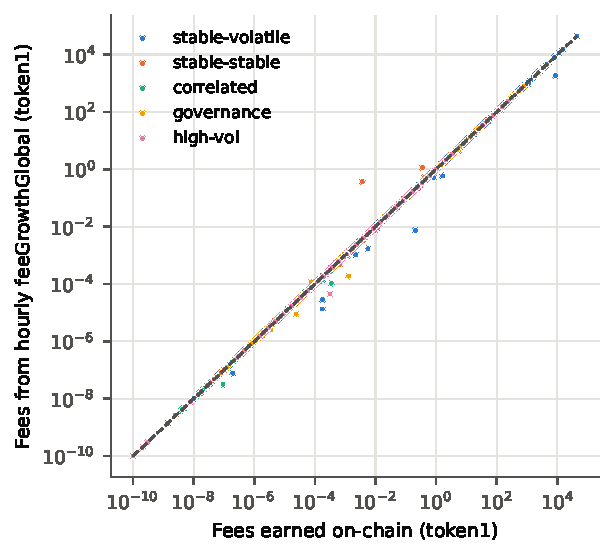
\includegraphics[width=0.8\columnwidth]{generated/fig_fee_validation.pdf}
\caption{Fees predicted from the hourly pool accumulators (Eq.~\eqref{eq:fee_growth}) versus the fees recorded on-chain for real full-range positions, per interval between position updates (log scale).}
\label{fig:fee_validation}
\end{figure}


\section{Empirical Results}
\label{sec:results}

\subsection{Correlation Lowers IL, Competition Lowers Fees}
\label{subsec:fees_vs_divergence}

\begin{table}[t]
\centering
\scriptsize
\setlength{\tabcolsep}{2.5pt}
\begin{tabular}{@{}lrrrrrrr@{}}
\toprule
Category & $n$ & Fee & IL & $-\sigma^2/8$ & $P_{10}$ IL & Net & Corr. \\
\midrule
Stable--volatile & 556 & 0.449 & -0.454 & -0.398 & -1.43 & -0.005 & 0\% \\
Stable--stable & 179 & 0.010 & 0.000 & -0.001 & 0.00 & 0.010 & -- \\
Correlated & 261 & 0.087 & -0.073 & -0.059 & -0.21 & 0.014 & 91\% \\
Governance & 349 & 0.673 & -0.432 & -0.448 & -1.05 & 0.242 & 69\% \\
High-vol./declining & 222 & 1.176 & -0.811 & -0.813 & -1.74 & 0.365 & 56\% \\
\bottomrule
\end{tabular}

\caption{Monthly full-range outcomes by category (\%, mean over pool-months with TVL $\geq$ 1M USD), namely fee yield, realized IL, LVR prediction, 10th-percentile IL and net yield over HODL. Corr.\ is the share of the individual token variances that correlation offsets in Eq.~\eqref{eq:pair_variance}.}
\label{tab:categories}
\end{table}

Table~\ref{tab:categories} summarizes the monthly full-range outcomes by category. The LVR prediction of Eq.~\eqref{eq:lvr} closely matches the realized IL. Across all pool-months, the mean IL is \MeanIL{} against a predicted \MeanPredIL{}, and a regression of the realized IL on the prediction has a slope of \LvrSlope{} ($R^2=\LvrRsq$). Correlation is the main driver of the differences in IL across pools. For correlated pairs, the covariance term of Eq.~\eqref{eq:pair_variance} offsets \CorrOffset{} of the individual token variances (mean $\rho=\CorrRho$). Hence, their IL is several times smaller than that of stable--volatile pairs, as shown in Fig.~\ref{fig:variance_decomposition}.

However, fee income falls by a similar factor. Correlated and stablecoin pairs mostly trade at low fee tiers against deep liquidity, so their fee yield is a small fraction of that of volatile pairs. After subtracting IL, they earn close to zero. Stable--volatile pools lose to HODL on average despite their large fee income, in line with the LVR literature~\cite{milionis2022automated}. On the other hand, governance and high-volatility pools earn the highest net yields, at the cost of deep tails. To conclude, lower IL is not by itself a reason to prefer a pool, since LPs compete for low-risk pools until their fee income roughly matches the risk.

\begin{figure}[t]
\centering
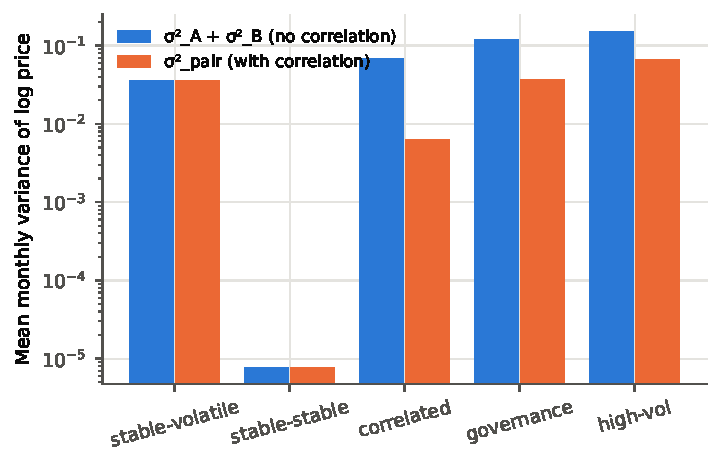
\includegraphics[width=0.9\columnwidth]{generated/fig_variance_decomposition.pdf}
\caption{Mean monthly variance of the log price per category, comparing the sum of the individual token variances with the pair variance of Eq.~\eqref{eq:pair_variance}. Stablecoins are priced at their peg, so stable pairs show no offset.}
\label{fig:variance_decomposition}
\end{figure}

\subsection{Calibration of Tail Forecasts}
\label{subsec:backtesting_il}

We next test whether the tail forecasts remain valid out of sample. For each pool and month $t$, starting at $t=13$, we forecast the 10th percentile of the next-month IL using only data prior to month $t$. The forecast uses either a rolling 12-month window or an expanding window. We then compute the exceedance rate $\hat{\alpha}$, namely the fraction of out-of-sample months in which the realized IL was worse than the forecast. We compare it with the target $q=0.10$ using two standard tests. The unconditional coverage test of Kupiec~\cite{kupiec1995techniques} checks whether $\hat{\alpha}$ equals $q$, and the independence test of Christoffersen~\cite{christoffersen1998evaluating} checks whether exceedances cluster in time.

Table~\ref{tab:calibration} reports the pooled results. With the 12-month window used by the selection rule, the model-based tail of Eq.~\eqref{eq:model_tail} has an exceedance rate of \ModelTailRate{} and passes both tests (Kupiec $p=\ModelTailKupiec$). On the other hand, the empirical 10th percentile under-covers (\EmpTailRate{}), and the Net90 bound fails clearly (\NetTailRate{}). With an expanding window, the model tail becomes conservative and the empirical percentile is better calibrated in aggregate, but its exceedances cluster in time. To conclude, the model-based tail is a valid risk forecast at the horizon and window used for pool selection.

\begin{table}[t]
\centering
\scriptsize
\setlength{\tabcolsep}{3pt}
\begin{tabular}{@{}llrcrr@{}}
\toprule
Forecast & Win. & Rate & 95\% CI & Kupiec & Christ. \\
\midrule
Model tail (ours) & 12m & 10.6 & [9.1, 12.4] & 0.461 & 0.347 \\
Model tail (ours) & exp. & 7.7 & [6.3, 9.2] & 0.003 & 0.058 \\
Empirical $P_{10}$ & 12m & 15.9 & [14.0, 18.0] & $<$0.001 & 0.716 \\
Empirical $P_{10}$ & exp. & 10.8 & [9.2, 12.6] & 0.359 & 0.026 \\
Net90 bound & 12m & 20.2 & [18.1, 22.4] & $<$0.001 & $<$0.001 \\
Net90 bound & exp. & 16.6 & [14.7, 18.7] & $<$0.001 & $<$0.001 \\
\bottomrule
\end{tabular}

\caption{Pooled out-of-sample calibration of 10th-percentile forecasts (target exceedance rate 10\%). The columns give the exceedance rate (\%), its Wilson 95\% interval and the $p$-values of the Kupiec and Christoffersen tests.}
\label{tab:calibration}
\end{table}

\subsection{Out-of-Sample Pool Selection}
\label{subsec:selection}

\textbf{Setup.} At the start of each month from June~2022, we score every eligible pool using only data from before the decision. We then hold the top $k\in\{1,3,5\}$ pools with equal weights for one month, for a total of \NDecisions{} decisions. A pool is eligible if it has at least 12 months of history and a TVL of at least 1M USD at the decision time, which leaves \EligibleMin{}--\EligibleMax{} pools per month. Opening a position costs the entry gas plus a swap of half the deposit at the pool's fee, and closing it costs the exit gas. The capital is 100K USD, and returns are measured over HODL of the deposited tokens.

We compare $S_\lambda$, for a grid of $\lambda$ values fixed in advance, with several baselines. These are Net90, the highest median fee, the lowest variance (the pure LVR ranking), equal weights over all eligible pools and random top-$k$ portfolios. The information coefficient (IC) measures how well a score ranks the pools. It is the monthly Spearman rank correlation between the score and the realized net yield across eligible pools, where 1 means a perfect ranking and 0 means no information. Its $t$-statistic uses Newey--West standard errors~\cite{newey1987simple}, which account for the dependence between consecutive months.

\begin{figure*}[t]
\centering
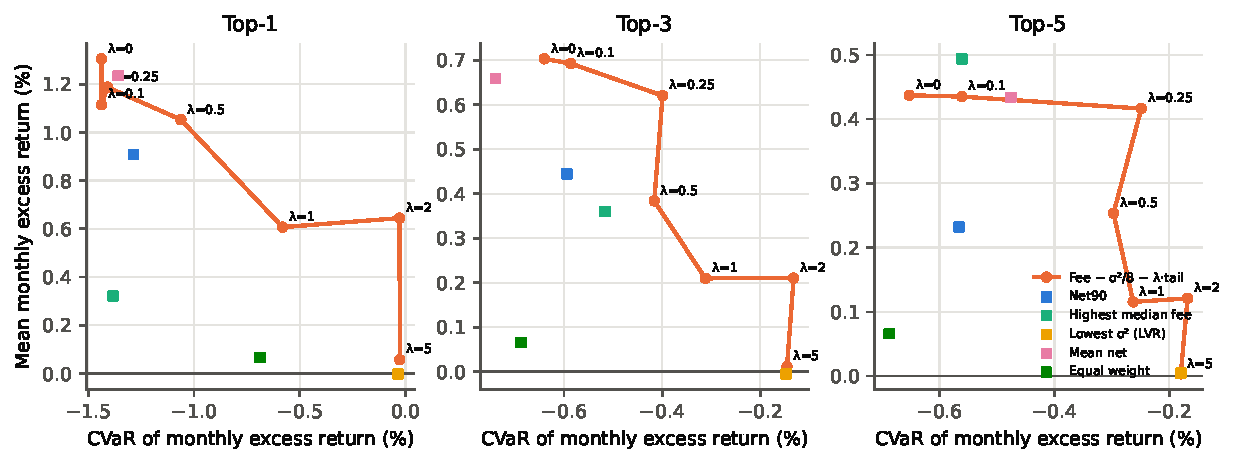
\includegraphics[width=\textwidth]{generated/fig_frontier.pdf}
\caption{Out-of-sample risk--return frontier, showing the mean monthly excess return over HODL after costs against its CVaR at 10\% for the mean--tail family $S_\lambda$ ($\lambda=0$ is fee $-\,\sigma^2/8$) and the baselines.}
\label{fig:frontier}
\end{figure*}

\begin{table}[t]
\centering
\scriptsize
\setlength{\tabcolsep}{2.2pt}
\begin{tabular}{@{}lrrrrrrr@{}}
\toprule
 & & \multicolumn{2}{c}{$k=1$} & \multicolumn{2}{c}{$k=3$} & \multicolumn{2}{c}{$k=5$} \\ \cmidrule(lr){3-4}\cmidrule(lr){5-6}\cmidrule(lr){7-8}
Strategy & IC & Mean & CVaR & Mean & CVaR & Mean & CVaR \\
\midrule
Fee $-\,\sigma^2/8$ ($\lambda{=}0$) & 0.27 & 1.31 & -1.44 & 0.70 & -0.64 & 0.44 & -0.65 \\
\quad $\lambda=0.1$ & 0.13 & 1.11 & -1.44 & 0.69 & -0.59 & 0.44 & -0.56 \\
\quad $\lambda=0.25$ & 0.01 & 1.19 & -1.41 & 0.62 & -0.40 & 0.42 & -0.25 \\
\quad $\lambda=0.5$ & -0.09 & 1.05 & -1.06 & 0.38 & -0.42 & 0.25 & -0.30 \\
\quad $\lambda=1$ & -0.17 & 0.61 & -0.58 & 0.21 & -0.31 & 0.12 & -0.26 \\
\quad $\lambda=2$ & -0.21 & 0.64 & -0.03 & 0.21 & -0.13 & 0.12 & -0.17 \\
\quad $\lambda=5$ & -0.25 & 0.06 & -0.03 & 0.01 & -0.15 & 0.00 & -0.18 \\
Net90 & -0.09 & 0.91 & -1.29 & 0.44 & -0.59 & 0.23 & -0.57 \\
Highest median fee & 0.34 & 0.32 & -1.38 & 0.36 & -0.52 & 0.49 & -0.56 \\
Lowest $\sigma^2$ & -0.27 & 0.00 & -0.04 & 0.00 & -0.15 & 0.00 & -0.18 \\
Equal weight & -- & 0.07 & -0.69 & 0.07 & -0.69 & 0.07 & -0.69 \\
Random $k$ pools & -- & -0.06 & -- & -0.08 & -- & -0.10 & -- \\
\bottomrule
\end{tabular}

\caption{Out-of-sample selection results, with the IC of each score and the mean and CVaR at 10\% of the monthly excess return over HODL after costs (\%) when holding the top $k$ pools.}
\label{tab:selection}
\end{table}

\textbf{Ranking.} Table~\ref{tab:selection} and Fig.~\ref{fig:frontier} present the results. The expected net yield $S_0=\overline{y^{\mathrm{fee}}}-\overline{\sigma^2}/8$ ranks next-month outcomes with an IC of \IcLvr{} ($t=\IcLvrT$). Additionally, every fee-aware score beats random portfolios, which lose to HODL on average. Scores that only penalize divergence rank the pools in the wrong order. The lowest-variance ranking has an IC of \IcLowVar{}, and Net90, whose tail term dominates its fee term, has an IC of \IcNetTail{} ($t=\IcNetTailT$). Both favor correlated and stablecoin pools, which earn close to nothing as shown in Section~\ref{subsec:fees_vs_divergence}.

\textbf{Risk--return tradeoff.} We measure the downside risk by the CVaR at 10\%, namely the mean return of the worst 10\% of months. Increasing $\lambda$ moves the portfolio along a risk--return frontier (Fig.~\ref{fig:frontier}). Small values substantially cut the CVaR and the drawdown while keeping most of the expected return. Large values converge to the near-zero-return pools favored by the lowest-variance ranking. For $k\in\{3,5\}$, members of the family with a small $\lambda$ have both a higher mean and a smaller loss in the worst months than Net90. In paired block-bootstrap tests~\cite{kunsch1989jackknife}, Net90 underperforms $S_\lambda$ with $\lambda\le0.5$ at the 5\% significance level in \NLvrTestsSig{} of \NLvrTests{} comparisons, and it is never significantly better. We report the full frontier rather than a single $\lambda$, since the choice of $\lambda$ reflects the risk preference of the LP.

\subsection{Robustness}
\label{subsec:robustness}
\textbf{Sensitivity.} We repeat the comparison between the empirical tail score and $S_0$ over \NSensCells{} parameter combinations. These vary the tail level ($q\in\{0.05,0.10,0.20\}$), the horizon (14 days, one month and two months), the calibration window (6 months, 12 months and expanding) and $k$. The empirical tail score has a lower mean return than $S_0$ in \NSensNetTailBehind{} of the \NSensCells{} cells. Fig.~\ref{fig:sensitivity} shows the differences for $k=\SensitivityK$.

\begin{figure}[t]
\centering
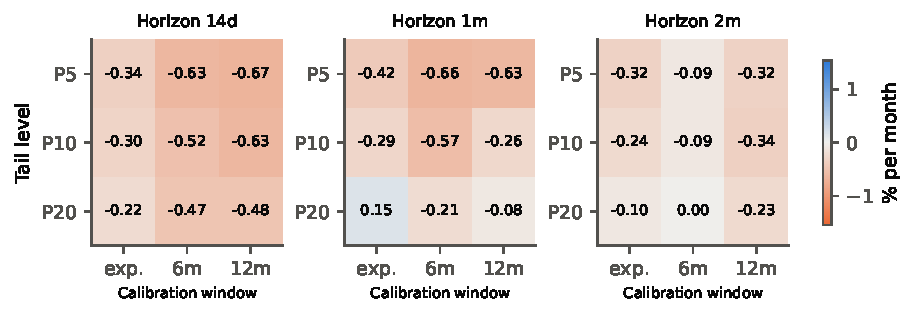
\includegraphics[width=\columnwidth]{generated/fig_sensitivity.pdf}
\caption{Sensitivity of the comparison for $k=\SensitivityK$. Each cell shows the mean excess return of the empirical tail score (median fee plus $q$-quantile IL) minus that of $S_0$, in \% per month, per tail level, calibration window and horizon. Negative values (orange) favor $S_0$.}
\label{fig:sensitivity}
\end{figure}

\textbf{Concentrated ranges.} We repeat the evaluation for passive positions with fixed ranges around the entry price, from $\pm1\%$ to $\pm20\%$, and with ranges of $\pm1\sigma$ to $\pm3\sigma$ for the trailing volatility $\sigma$. As in Section~\ref{subsec:fee_accounting}, we credit the fee-growth accumulators only in hours in which the price is in range. The full-range score $S_0$ remains informative for concentrated positions, and more so for wider ranges (Fig.~\ref{fig:ic_by_range}). Its IC against the realized concentrated net yield rises from \IcRangeOne{} for $\pm1\%$ and \IcRangeFive{} for $\pm5\%$ to \IcRangeTwenty{} for $\pm20\%$. For ranges scaled to the trailing volatility, the IC is \IcRangeSigmaMin{}--\IcRangeSigmaMax{}. For the narrowest range, tail aversion helps, since volatile pools leave a narrow range quickly. At $\pm1\%$, the IC rises to \IcRangeOneTail{} for $\lambda=\LamMax$. On the other hand, Net90 has an IC of at most \IcRangeNetTailMax{} for the wider and the volatility-scaled ranges. Passive fixed ranges lose to HODL on average, with a mean net yield of \NetRangeOne{} per month at $\pm1\%$ and \NetRangeTwenty{} at $\pm20\%$. Volatility-scaled ranges roughly break even (\NetRangeSigma{} at $\pm\SigmaRangeMax\sigma$). Hence, the range choice remains a separate decision after pool screening.

\begin{figure}[t]
\centering
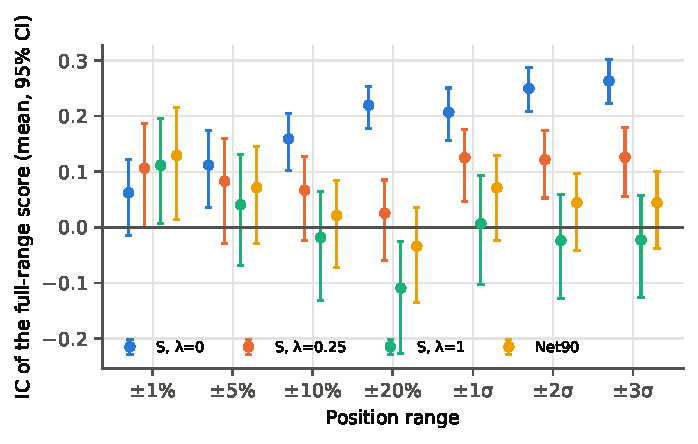
\includegraphics[width=\columnwidth]{generated/fig_ic_by_range.pdf}
\caption{IC of full-range scores against the realized net yield of passive concentrated positions, per range (mean and 95\% block-bootstrap interval).}
\label{fig:ic_by_range}
\end{figure}

\textbf{Persistence.} The daily log price ratio is highly persistent. We measure this by the AR(1) half-life, namely the time it takes a deviation of the ratio to shrink by half. Across pools, the mean half-life over rolling 180-day windows ranges from \HalfLifeMin{} to \HalfLifeMax{} days. Hence, divergence episodes typically outlast a one-month holding horizon, and a monthly rebalancing rule cannot rely on mean reversion within the horizon.
\arad{Add the Arbitrum out-of-sample replication (E11) here if it is run.}


\section{Scope and Implications of LP Screening}
\label{sec:discussion}

The empirical analysis positions the proposed score as a general screening layer for LPs rather than a strategy model specific to Uniswap v3. We next discuss three implications.

\subsection{From Divergence Metrics to Pool Screening}

A key empirical finding is that divergence risk stems from the dynamics of the relative price rather than from the volatility of each token alone. Correlated pairs exhibit much lower IL than stable--volatile pairs, and Eq.~\eqref{eq:pair_variance} quantifies this effect. However, this does not make correlated pools superior, since fee generation adjusts to the risk. Hence, pool screening must weigh fees against divergence, and the LVR rate provides the natural exchange rate between the two. Downside-aware terms remain important, as average outcomes can mask severe tail dislocations. Still, the tail should be forecast from a model with enough data, and weighted by an explicit risk aversion rather than added at full weight to a typical fee.

\subsection{Fee Velocity Rather Than Fee Tier}

The fee tier alone is insufficient for assessing LP compensation. For instance, a 0.05\% pool requires six times the turnover of a 0.30\% pool to match its fee yield. Hence, \emph{fee velocity} is the relevant screening quantity,
\[
y^{\mathrm{fee}}_t
\approx
\mathrm{FeeTier}
\cdot
\frac{\mathrm{Volume}_t}{\mathrm{TVL}_t}.
\]
This expression separates the fee margin per unit of volume from the turnover of the capital. High volume does not ensure high turnover when TVL is also large, and a high-fee pool can underperform when deep liquidity dilutes its fee yield. The fee-growth accounting of Eq.~\eqref{eq:fee_growth} measures this yield exactly for a full-range position.

\subsection{Implications for LP Strategy Design}

These findings suggest a two-stage design for LP strategies. First, the LP uses the proposed score to screen for pools with attractive fee--divergence profiles at its risk aversion. Next, it evaluates protocol-specific parameters such as range selection, active share, rebalancing, gas costs, slippage and path-dependent inventory exposure. The framework does not claim that full-range IL exactly values every concentrated position. Rather, it provides a general screening layer that complements detailed protocol-specific LP models.

\textbf{Limitations.} The fee model treats the position as a price taker, and the daily fee cap only bounds this effect. The subgraph prices major stablecoins at their peg, so USD-based statistics miss depeg episodes. IL and fees are not affected, as they are computed from the pool price. Finally, hourly data cannot resolve price moves within the hour, which matters for very narrow ranges.

\section{Conclusion}
\label{sec:conclusion}
In this paper, we developed a data-driven pool-screening framework that lets LPs weigh fee income against IL risk beyond simple fee-tier heuristics. For full-range positions, we showed that fees and divergence losses can be measured consistently from on-chain accumulators. The expected loss follows the LVR rate $\sigma^2_{\text{pair}}/8$, and a model-based tail forecast from hourly volatility is well calibrated. Across \NPools{} Uniswap v3 pools, correlation lowers IL as theory predicts, but fee competition removes most of the benefit. The fee-minus-loss score ranks pools well out of sample. Moreover, a small risk-aversion weight on the tail trades a modest part of the return for a substantially lower downside risk. Since the model also applies to Uniswap v2 and v4 pools, in future work we intend to extend the analysis to these protocols, additional networks and other AMM designs. Additionally, we intend to develop range-selection and adaptive fee policies that adjust to time-varying IL risk.



\bibliographystyle{IEEEtran}
\bibliography{references}

\end{document}
